\paragraph{}Los procesos que intervienen en dicho módulo son los siguientes:

\begin{description}
 \item[Validar asesor] Constará de los procedimientos necesarios para que se
      validen los datos de acceso permitiendo el acceso o no del asesor.
 \item[Procesar entrada] Constará de los procedimientos necesarios para que se
      mantenga la veracidad, integridad y consistencia de la base de datos así
      como la comprobación de la integridad de los datos introducidos por el
      asesor.
 \item[Administrar BBDD] Constará de los procedimientos necesarios para mantener
      toda la información de la base de datos, como por ejemplo las distintas
      reuniones que estableza un asesor.
 \item[Explotación del sistema]  Constará de los procedimientos necesarios para
      consultar datos de la aplicación.
 \item[Ayuda] Administra la documentación que sirve de ayuda en el manejo de
      esta aplicación.
 \item[Procesar salida] Constará de los procedimientos necesarios para que
      puedan ser visualizados los resultados de los procesos anteriores.
\end{description}

\paragraph{}La figura \ref{diagramaNivel2-Asesores} muestra el nivel de
abstracción 2: Asesores.

  \begin{figure}[!ht]
    \begin{center}
      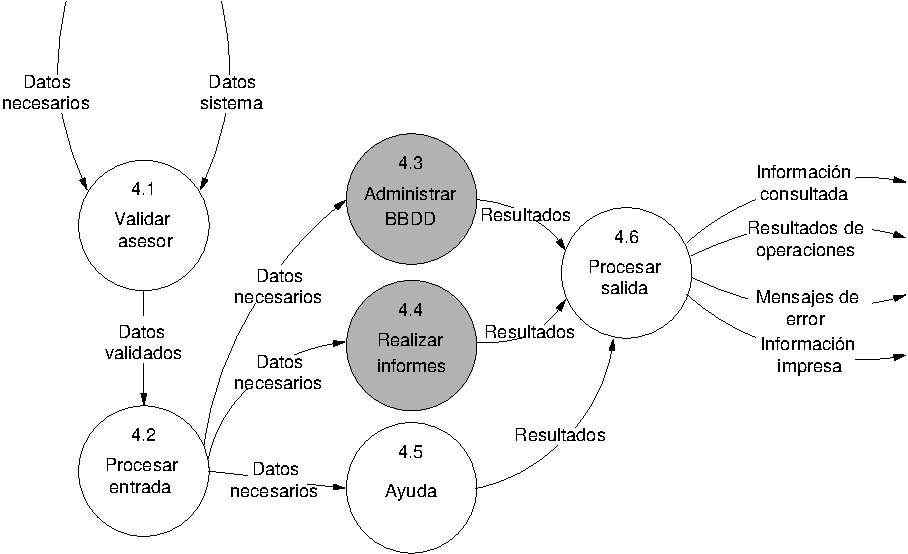
\includegraphics[]{08.Analisis_Funcional/8.2.DFDs/Niveles/Nivel2/Diagramas/nivel2-Asesores.pdf}
      \caption{Nivel de abstracción 2: Asesores.}
      \label{diagramaNivel2-Asesores}
    \end{center}
  \end{figure}